% begin module max-min-def
\begin{frame}[t]
\begin{columns}[c]
\column{.5\textwidth}
\ \only<-2,4,6-7,10>{%
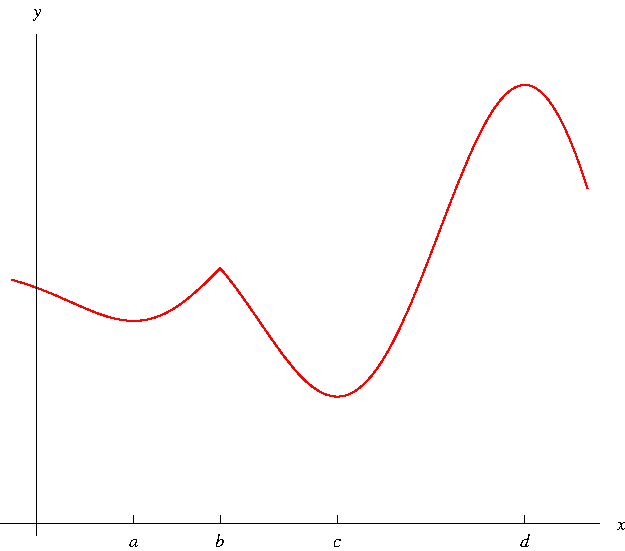
\includegraphics[width=5.5cm]{maxima-minima/pictures/04-01-minmaxa.pdf}%
}%
\only<handout:0| 3,9>{%
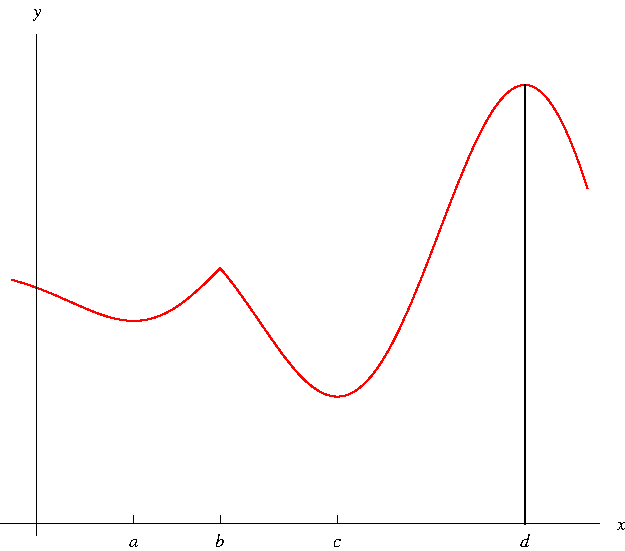
\includegraphics[width=5.5cm]{maxima-minima/pictures/04-01-minmaxe.pdf}%
}%
\only<handout:0| 5,12>{%
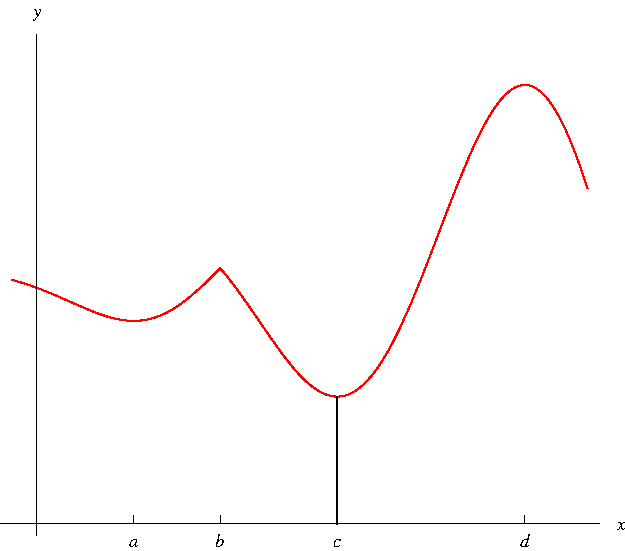
\includegraphics[width=5.5cm]{maxima-minima/pictures/04-01-minmaxd.pdf}%
}%
\only<handout:0| 8>{%
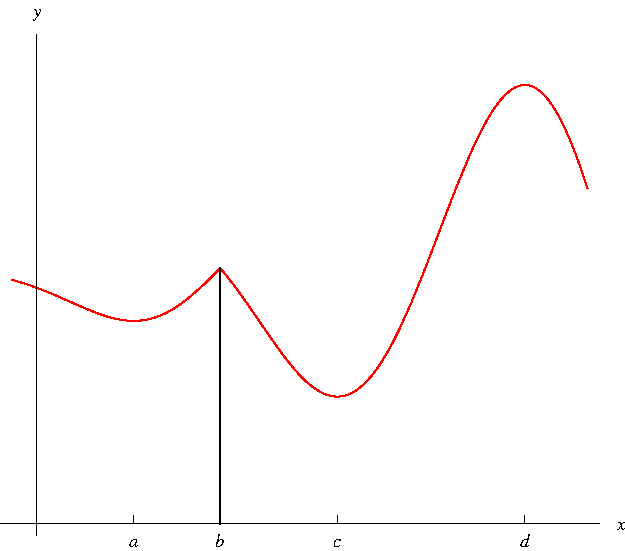
\includegraphics[width=5.5cm]{maxima-minima/pictures/04-01-minmaxc.pdf}%
}%
\only<handout:0| 11>{%
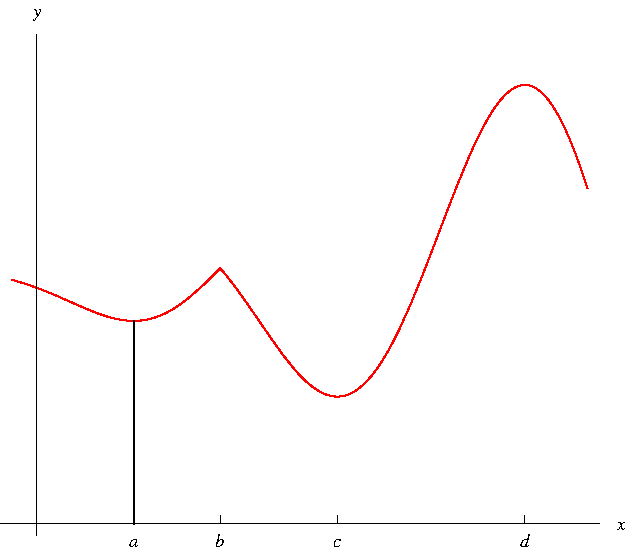
\includegraphics[width=5.5cm]{maxima-minima/pictures/04-01-minmaxb.pdf}%
}%
\column{.5\textwidth}
\begin{itemize}
\item<2-| alert@2-3>  Absolute maximum at \uncover<3->{$d$}
\item<2-| alert@4-5>  Absolute minimum at \uncover<5->{$c$}
\item<7-| handout:2| alert@7-9>  Local maximum at \uncover<8->{$b$} \uncover<9->{and $d$}
\item<7-| handout:2| alert@10-12>  Local minimum at \uncover<11->{$a$} \uncover<12->{and $c$}
\end{itemize}
\end{columns}
\only<handout:1| -5>{%
\begin{definition}[Absolute Maximum or Minimum]
A function $f$ has an absolute maximum (or global maximum) at $c$ if $f(c) \geq f(x)$ for all $x$ in the domain of $f$.  The number $f(c)$ is called the maximum value of $f$.

Likewise, $f$ has an absolute minimum at $c$ if $f(c) \leq f(x)$ for all $x$ in the domain of $f$.  $f(c)$ is called the minimum value of $f$.

Maximum and minimum values of $f$ are called extreme values.
\end{definition}
}%
\only<handout:2| 6->{%
\begin{definition}[Local Maximum or Minimum]
A function $f$ has a local maximum at $c$ if $f(c) \geq f(x)$ for all $x$ in some open interval containing $c$.  Similarly, $f$ has a local minimum at $c$ if $f(c) \leq f(x)$ for all $x$ in some open interval containing $c$.
\end{definition}
}%
\end{frame}
% end module max-min-def
